\documentclass{article}
\usepackage[utf8]{inputenc}
\usepackage{graphicx}
\usepackage{cleveref}

\title{First IDP Report}
\author{Group M213 ; Team 213 ; Robot 213}
\date{November 2022}

% To be confirmed that it requires the setspace package, try with and without.
\usepackage{setspace}

% Let top 85% of a page contain a figure
\renewcommand{\topfraction}{0.85}

% Default amount of minimum text on page (Set to 10%)
\renewcommand{\textfraction}{0.1}

% Only place figures by themselves if they take up more than 75% of the page
\renewcommand{\floatpagefraction}{0.75}

%zet de bladspiegel :
\setlength\paperwidth{20.999cm}\setlength\paperheight{29.699cm}\setlength\voffset{-1in}\setlength\hoffset{-1in}\setlength\topmargin{1.499cm}\setlength\headheight{12pt}\setlength\headsep{0cm}\setlength\footskip{1.131cm}\setlength\textheight{25cm}\setlength\oddsidemargin{2.499cm}\setlength\textwidth{16.5cm}

\begin{document}

\maketitle

% TODO: Please fill in your details in the table below

\begin{table}[]
    \centering
    \begin{tabular}{|c|c|c|c|}
        \hline
        Name &  CRsid & College & Lab Group \\
        \hline
        Matthew Hendricks & mah237 & Pembroke & 35 \\
        Louis Pender & lwp256 & & \\
        Hor Ye Heng & yhh35 & & \\
        Wen Yian & yw543 & & \\
        Ian & & & \\
        Yuge & & & \\
        \hline
    \end{tabular}
    \caption{Coversheet information}
    \label{tab:Coversheet}
\end{table}


\newpage

\section{Introduction}
\quad TODO: Include overall system Level Diagram and overall approach to solve the problem


\section{Project Management}
\quad L.W. Pender was selected as the leader of the group. We created a Trello project which has functionalities like a Gantt chart and Kanban boards as our project management systems. We made a rough timeline of the large milestones of the project such as having a fully assembled robot, having the sensors all attached onto the robot and funcitoning, having a working robot and testing, and placed these onto the Trello project. We then made smaller short-term goals for each team to achieve.
    
\section{Mechanical}
\quad The mechanical team consists of Pender, L.W. (lwp26) and Hendricks, M.A. (mah237). Our short term plan for the mechanical team was to get a good CAD model and a cardboard model out for the robot by the 14th of November. We started off by making some design decisions.

\subsection{Drive System}
\quad \quad We initially considered a few drive systems for the robot, namely a 3-wheeled differential drive system, a 4-wheeled tank drive system, making our ownn Mecanum wheels and a simple 2-wheeled system. 

\quad We ruled out the Mecanum wheels idea due to the sheer difficulty of manufacturing such a wheel without much added benefit to the project since the main priority for our team would be rapid production so that testing can begin sooner rather than later. The 3-wheeled differential drive was also ruled out due to not having 3 same-sized wheels. This is because we don't want the base of the chassis to be inclined in case we would have markers (such as QR codes) used by the software team for navigation and other purposes. The inclination would probably lead to larger errors in navigation. We ruled out the 4-wheeled tank drive system, as we were worried about slipping occuring in one of the sets of wheels if the ratios of the speeds were not accurate. This is especially important to us since we're thinking about using a light sensor as a rotary encoder to have an accurate measure of the distance travelled by the robot. A table summarising our comparisons can be seen in \Cref{tab:drive_comp}.

\quad Therefore, the best option we settled on was the simple 2-wheeled system, since it would be the simplest to manufacture. We plan to use the larger wheels so that our rotary encoder would be more accurate. The wheels will be connected to the higher torque lower RPM motor via the given motor adaptors. The higher torque will help in the robot going up the ramp. The motors will be attached to the robot by a metal bracket and bolting it onto the threads on the aluminium plate on the motor. We also will place a ball castor at the other end of the chassis to ensure the robot remains stable as it ascends the ramp.

\begin{table}[]
    \centering
    \begin{tabular}{|c|p{5cm}|p{5cm}|}
        \hline
        Idea & Advantages & Disadvantages \\
        \hline
        2-wheeled + Castor wheel & Fast to manufacture quickly& Might be harder to turn \\
        3-wheeled differential-drive & Easy to manufacture quickly & Might slip since wheels are not of same size \\
        4-wheeled tank drive system & Very reliable & More motors required and hard to sync the motor's rpm ratio due to different sized wheels \\
        \hline
    \end{tabular}
    \caption{Drive System Comparison}
    \label{tab:drive_comp}
\end{table}

\subsection{Chassis}
\quad After looking at the sizes of the various components (such as the Arduino and the battery pack) that we needed to fit onto the chassis we make a rough guess of a dimension of the base of the chassis to be $250mm \times 140mm$.

The chassis design for the prototype has been designed to be very modular, we have multiple holes for the components fitting locations so that we can swap the positions of the sensors and other components easily to redistribute the mass in the robot. We have laser cutted out parts of the chassis and are currently assembling the robot.

\subsection{Gripping Mechanism}
\quad We had 3 main ideas on how to capture the block. 

\quad The first was a simple pushing idea where we had a slight protrusion at the edges of the robot to ensure it doesn't get pushed off the robot. However this not only limits our route to be leaving the collection arena from the tunnel, it also is not reliable during turning.

\quad The second idea was to have a rack and pinion powering a moving stick to move closer to another stationary stick to grab the block. The problem with this was that the rack and pinion mechanism is less reliable and the block will be gripped to one side of the mechanism and the mass distribution will be shifted.

\quad The idea we settled on was to use a scissor like gripping mechanism as shown in \Cref{fig:grip_mech}. This might have slightly more parts but it is more reliable than the rack and pinion and the center of mass is not affected.

\subsection{Cardboard Model and CAD}
\quad We have made a cardboard model prototype for testing purposes as can be seen in \Cref{fig:cardboard_model}.
% Louis Could you please add some photos of the CAD and reference them in this section thank you.

\section{Electrical}



\section{Software}


\section{Appendix}
% Please put all of your image documents in the asset folder and place all of your figures here. TQ
\begin{figure}
    \centering
    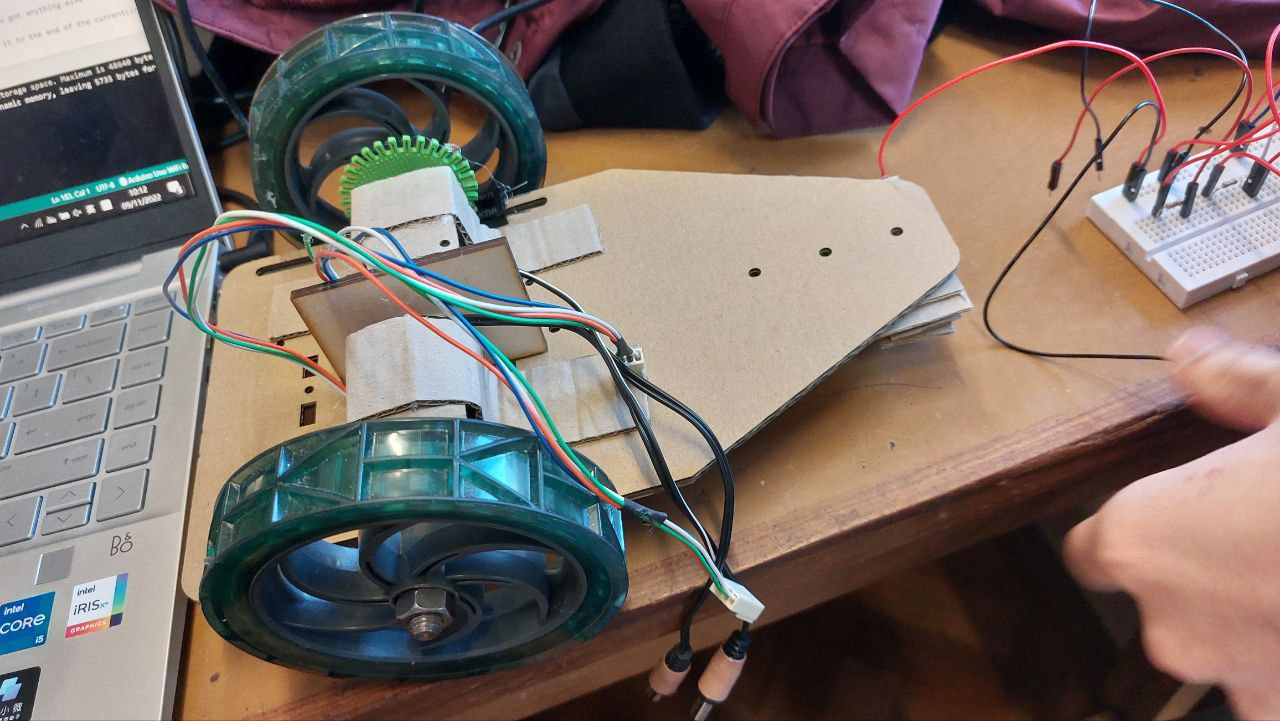
\includegraphics[width=0.8\textwidth]{assets/Cardboard_model.jpg}
    \caption{Cardboard Model}
    \label{fig:cardboard_model}
\end{figure}

\begin{figure}
    \centering
    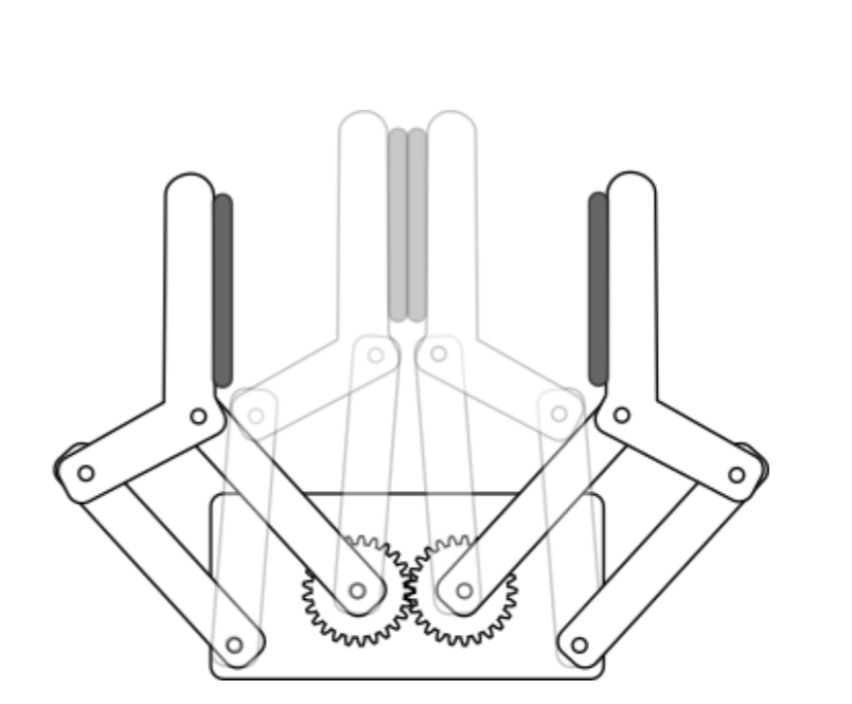
\includegraphics[width=0.8\textwidth]{assets/Gripper_Mechanism.jpg}
    \caption{Scissor-like Gripper Mechanism}
    \label{fig:grip_mech}
\end{figure}


\end{document}
